\section{Related work}
\label{qoala:sec:related_work}

Networks of quantum processors have been realized using different quantum hardware platforms including, for example, nitrogen-vacancy (NV) centers in diamond~\cite{pompili2021realization}, and trapped ions~\cite{krutyanskiy2023entanglement}.
A first operating system QNodeOS~\cite{donne_design_2024} (see also \cref{chp:qnodeos}) including a network stack~\cite{pompili2022experimental} has been designed and implemented on real quantum network nodes based on NV centers in diamond.
QNodeOS makes use of the NetQASM execution framework~\cite{dahlberg2022netqasm} (see also \cref{chp:netqasm}), where a classical network processing unit (CNPU) dispatches NetQASM routines for execution by a quantum network processing unit (QNPU).
This meant, e.g., that QNodeOS was unable to have any scheduling control over the joint classical-quantum execution, which could lead to a failure in executing programs successfully.
Our work builds on top of ideas of QNodeOS and NetQASM, but addresses critical challenges that were not handled by these previous systems, including the ability to schedule hybrid programs and to optimize over the whole program code (see \cref{qoala:fig:qoala_vs_qnos} for a comparison).
Building on the only such systems that have seen real world implementation on quantum hardware, opens the door for a later implementation of Qoala on quantum hardware by implementing an improved low-level classical control hardware architecture (\cref{qoala:sec:architecture}).

\begin{figure}[t]
    \centering
    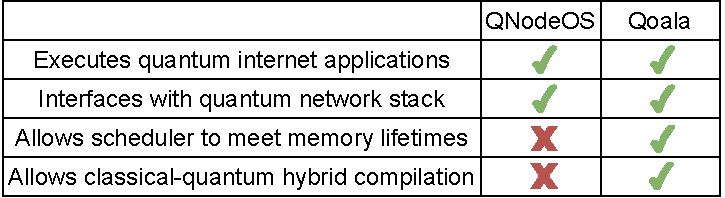
\includegraphics[width=0.7\textwidth]{figures/qoala/qoala_vs_qnos.pdf}
    \caption{
        QNodeOS (\cref{chp:qnodeos}) vs. Qoala capabilities.
    }
    \label{qoala:fig:qoala_vs_qnos}
\end{figure}

Research has been done on related topics, such as distributed quantum computing, or hybrid (non-interactive) quantum computing. Hybrid classical-quantum programs have been extensively studied in quantum computing, e.g. in the context of \textit{variational quantum eigensolvers (VQE)}~\cite{diadamo2021distributed, liu2022layer} or \textit{quantum approximate optimization algorithms (QAOA)}~\cite{farhi2014quantum}. However, they differ in two important aspects: although they are hybrid, they are not \textit{interactive} during the quantum execution:
(1) classical and quantum segments do not run concurrently, but quantum segments are executed in their entirety before returning to classical segments, i.e. no quantum state is kept in the processor between the execution of different quantum segments.
(2) such hybrid programs lack network interoperability (entanglement generation and classical message-passing between nodes), and also do not have the same timing and flexibility requirements.

Distributed quantum computing~\cite{cacciapuoti2019quantum} shares similarities with quantum internet applications but differs in several aspects.
In the former, complete control is assumed over all participating nodes, such as an application distributed across multiple cores on a single chip~\cite{ovide2023mapping, jnane2022multicore}.
Generally, the capabilities of each core and the latencies between them are fully known, allowing for precise scheduling and orchestration of individual programs running on each core to optimize overall execution.
In contrast, programs in quantum internet applications operate independently (and may even be running on different quantum hardware); therefore they have a degree of autonomy in their own scheduling, and are not fully aware of the actions or timing of other programs.

Entanglement distribution in networks is another related topic that has been extensively studied (see e.g. surveys~\cite{wei2022towards, azuma2021tools}).
However, these works do not deal with executing network applications, and give only predictions for applications in which entanglement is immediately measured (e.g. QKD).

The concept of (soft) deadlines for program execution is of course well known from classical real-time systems that are often used in domains where deterministic and time-critical response is essential, such as automotive, aerospace and medical devices~\cite{liu1973scheduling, hambarde2014survey, buttazzo2011hard}, including examples of systems with mixed timing precision~\cite{burns2017survey}.
We draw inspiration from this domain, and the present architecture opens the door to explore algorithms and concepts from this domain to be applied to the execution of quantum internet applications.
